\chapter{Supporting Information for Supramolecular Interactions of Group VI Metal Carbonyl Complexes: the Facilitating Role of 1,3-bis(\textit{p}-isocyanophenyl)urea}
\label{chap:supra_SI}

%---------------------------------------------
\newpage % NOTE: The appendix title should be on its own page.
%---------------------------------------------

\begin{figure}
    \centering
    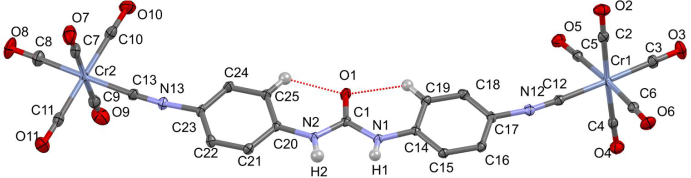
\includegraphics[width=0.8\linewidth]{figures/pub2/si_fig1.png}
    \caption{Molecular structure of complex \textbf{2}. Thermal ellipsoids are rendered at the 50\% probability level. Only urea N–H atoms and aromatic hydrogen atoms participating in hydrogen bonding are shown.}\label{fig:complex2}
\end{figure}

\begin{figure}
    \centering
    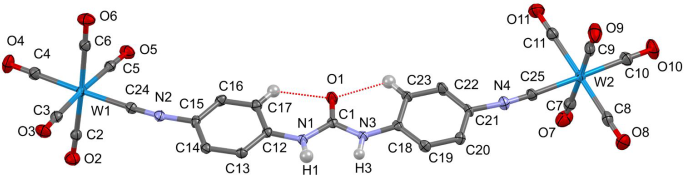
\includegraphics[width=0.8\linewidth]{figures/pub2/si_fig2.png}
    \caption{Molecular structure of complex \textbf{4}. Thermal ellipsoids are rendered at the 50\% probability level. Only urea N–H atoms and aromatic hydrogen atoms participating in hydrogen bonding are shown.}\label{fig:complex4}
\end{figure}

\section{Electrochemical Measurements}

Cyclic voltammograms were recorded in 0.1 M [Bu$_{4}$N][PF$_{6}$] DMF solutions at $\nu$ = 100 mV/sec with a Princeton Applied Research VersaSTAT 3 potentiostat. All experiments were performed using a standard three-electrode configuration under an atmosphere of pure nitrogen. Glassy carbon working electrodes (3 mm, CH Instruments) were used for all measurements and were polished with aqueous slurries of 0.3 $\mu$m and 0.05 $\mu$m alumina powder, sequentially. After polishing, the electrodes were rinsed with Milli-Q water, methanol, and dichloromethane and dried in a stream of air. Working electrodes were preconditioned by performing three cyclical scans from 2.0 to -2.5 V at 250 mV/sec in a DMF solution of [Bu$_{4}$N][PF$_{6}$] (0.1 M). A graphite rod served as the counter electrode and a silver wire immersed in a 0.1 M DMF solution of [Bu$_{4}$N][PF$_{6}$] and separated from the cell compartment by a porous glass frit (CoralPor 1000) was employed as a Ag$^{+}$/Ag pseudoreference electrode. Measured potentials are reported relative to the ferrocenium(1+)/ferrocene(0) redox couple, which was achieved by addition of ferrocene at the end of each set of scans.

\begin{figure}
    \centering
    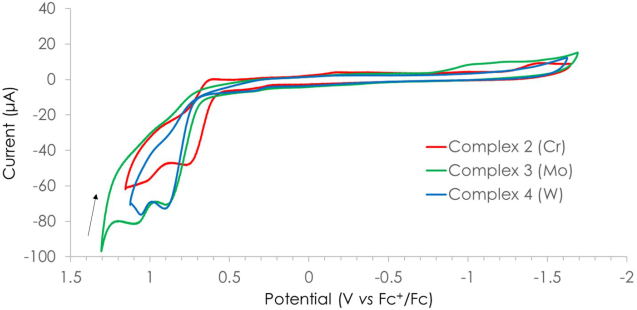
\includegraphics[width=0.8\linewidth]{figures/pub2/si_fig3.png}
    \caption{Cyclic voltammograms of complexes \textbf{2}-\textbf{4} ($\approx$ 1 mM) recorded in 0.1 M [Bu$_{4}$N][PF$_{6}$] DMF solution at $\nu$ = 100 mV/sec with a glassy carbon working electrode, graphite rod counter electrode, and a silver wire pseudoreference electrode.}\label{fig:cv}
\end{figure}


\begin{table}[]
\centering
\caption{X-ray data collection and refinement parameters for complexes \textbf{2}-\textbf{4}.} \label{tab:xray}
\begin{tabular}{lccc}
\hline
\textbf{Compound} & \textbf{2} & \textbf{3} & \textbf{4} \\ \hline
Formula & \makecell{C$_{25}$H$_{10}$N$_{4}$O$_{11}$Cr$_{2}$ \\ $\cdot$CH$_{3}$CN} & \makecell{C$_{25}$H$_{10}$N$_{4}$O$_{11}$Mo$_{2}$ \\ $\cdot$CH$_{3}$CN} & \makecell{C$_{25}$H$_{10}$N$_{4}$O$_{11}$W$_{2}$ \\ $\cdot$CH$_{3}$CN} \\
Formula weight & 687.42 & 775.30 & 951.12 \\
Temperature (K) & 100 & 100 & 100 \\
Crystal system & monoclinic & monoclinic & monoclinic \\
Space group & P2$_{1}$/c & P2$_{1}$/c & P2$_{1}$/c \\
\textit{a} (\AA) & 6.8126(2) & 6.8694(5) & 6.8575(4) \\
\textit{b} (\AA) & 13.8536(5) & 14.0047(10) & 13.9691(9) \\
\textit{c} (\AA) & 32.1439(11) & 32.536(2) & 32.525(2) \\
$\alpha$ (deg) & 90 & 90 & 90 \\
$\beta$ (deg) & 93.8630(10) & 93.115(2) & 93.145(2) \\
$\gamma$ (deg) & 90 & 90 & 90 \\
Volume (\AA$^{3}$) & 3026.82(17) & 3125.5(4) & 3110.9(3) \\
Z & 4 & 4 & 4 \\
density (g/cm$^{3}$) & 1.509 & 1.648 & 2.031 \\
abs coeff (mm$^{-1}$) & 0.784 & 0.867 & 7.454 \\
F(000) & 1384 & 1528 & 1784 \\
Crystal size (mm) & 0.42 × 0.18 × 0.12 & 0.4 × 0.05 × 0.05 & 0.17 × 0.14 × 0.05 \\
$\lambda$ (MoK$\alpha$) (\AA) & 0.71073 & 0.71073 & 0.71073 \\
2$\theta$ range (deg) & 5.87 to 55.068 & 5.818 to 61.12 & 5.804 to 54.968 \\
reflns (coll) & 40623 & 120953 & 50308 \\
reflns (unique) & 6937 & 9565 & 7120 \\
\makecell[l]{\rule{0pt}{2ex}Data/restraints/\\ ~~~parameters} & 6937/0/415 & 9565/0/415 & 7120/0/415 \\
GOF (on F$^{2}$) & 1.131 & 1.072 & 1.206 \\
\makecell[l]{\rule{0pt}{2ex}Final R indexes \\ ~~~ [I $\geq$ 2$\sigma$ (I)]} & \makecell{\rule{0pt}{2ex}R$_{1}$ = 0.0356, \\ ~~~ wR$_{2}$ = 0.0848} & \makecell{R$_{1}$ = 0.0327, \\ wR$_{2}$ = 0.0578} & \makecell{R$_{1}$ = 0.0242, \\ wR$_{2}$ = 0.0463} \\
\makecell[l]{\rule{0pt}{2ex}Final R indexes \\ ~~~ [all data]} & \makecell{R$_{1}$ = 0.0433, \\ wR$_{2}$ = 0.0877} & \makecell{R$_{1}$ = 0.0555, \\ wR$_{2}$ = 0.0623} & \makecell{R$_{1}$ = 0.0312, \\ wR$_{2}$ = 0.0477} \\
\makecell[l]{\rule{0pt}{2ex}Largest diff. \\ ~~~peak/hole (e \AA$^{-3}$)} & 0.45/-0.23 & 0.58/-0.47 & 0.88/-0.43
\end{tabular}
\end{table}


\begin{figure}
    \centering
    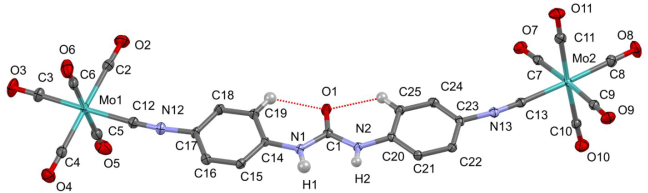
\includegraphics[width=0.8\linewidth]{figures/pub2/si_fig4.png}
    \caption{Atom labels used in structure analysis of complex \textbf{3} provided in \autoref{tab:bondlengths3}, \autoref{tab:angles3}, and \autoref{tab:dihedrals3}.}\label{fig:complex3-labels}
\end{figure}


\begin{table}[]
\centering
\caption{Heavy atom bond lengths (\AA) and RMSD for experimental X-ray and calculated crystal structures of complex \textbf{3}.} \label{tab:bondlengths3}
\begin{tabular}{lcl}
\textbf{Bond} & \textbf{exp.} & \textbf{DFT} \\ \hline
C12-Mo1 & 2.127 & 2.1778 \\
C14-C15 & 1.395 & 1.4104 \\
C14-C19 & 1.398 & 1.4094 \\
C15-C16 & 1.381 & 1.3892 \\
C16-C17 & 1.386 & 1.4013 \\
C17-C18 & 1.385 & 1.4021 \\
C18-C19 & 1.384 & 1.3907 \\
C20-C21 & 1.401 & 1.4084 \\
C20-C25 & 1.394 & 1.4085 \\
C21-C22 & 1.378 & 1.3885 \\
C22-C23 & 1.383 & 1.4003 \\
C23-C24 & 1.390 & 1.4038 \\
C24-C25 & 1.378 & 1.3904 \\
C26-C27 & 1.453 & 1.4564 \\
Mo1-C2 & 2.052 & 2.1024 \\
Mo1-C3 & 2.020 & 2.0675 \\
Mo1-C4 & 2.056 & 2.1078 \\
Mo1-C5 & 2.063 & 2.1201 \\
Mo1-C6 & 2.046 & 2.0903 \\
Mo2-C10 & 2.053 & 2.0989 \\
Mo2-C11 & 2.052 & 2.0963 \\
Mo2-C13 & 2.130 & 2.1826 \\
Mo2-C7 & 2.044 & 2.0925 \\
Mo2-C8 & 2.022 & 2.0745 \\
Mo2-C9 & 2.068 & 2.1158 \\
N1-C1 & 1.381 & 1.3827 \\
N1-C14 & 1.397 & 1.3956 \\
N12-C12 & 1.155 & 1.1747 \\
N12-C17 & 1.400 & 1.3832 \\
N13-C13 & 1.161 & 1.1749 \\
N13-C23 & 1.396 & 1.3825 \\
N2-C1 & 1.373 & 1.3840 \\
N2-C20 & 1.397 & 1.3958 \\
N3-C26 & 1.136 & 1.1619 \\
O1-C1 & 1.216 & 1.2293 \\
O10-C10 & 1.135 & 1.1509 \\
O11-C11 & 1.137 & 1.1506 \\
O2-C2 & 1.137 & 1.1495 \\
O3-C3 & 1.143 & 1.1560 \\
O4-C4 & 1.138 & 1.1488 \\
O5-C5 & 1.138 & 1.1472 \\
O6-C6 & 1.138 & 1.1524 \\
O7-C7 & 1.137 & 1.1496 \\
O8-C8 & 1.147 & 1.1550 \\
O9-C9 & 1.134 & 1.1463 \\ \hline
\textbf{RMSD} &  & \textbf{0.0279}
\end{tabular}
\end{table}


\begin{table}[]
\centering
\caption{Heavy atom bond angles (°) and RMSD for experimental X-ray and calculated crystal structures of complex \textbf{3}.} \label{tab:angles3}
\begin{tabular}{lcc}
\textbf{Bond Angle} & \textbf{exp.} & \textbf{DFT} \\ \hline
C1-N1-C14 & 127.10 & 127.47 \\
C1-N2-C20 & 128.00 & 128.30 \\
C10-Mo2-C11 & 176.44 & 178.47 \\
C10-Mo2-C13 & 92.66 & 91.79 \\
C11-Mo2-C13 & 90.38 & 89.43 \\
C12-N12-C17 & 172.00 & 170.06 \\
C13-N13-C23 & 171.90 & 171.30 \\
C14-C15-C16 & 120.90 & 120.95 \\
C14-C19-C18 & 119.70 & 119.87 \\
C15-C14-C19 & 119.30 & 119.19 \\
C15-C16-C17 & 119.10 & 119.29 \\
C16-C17-C18 & 120.80 & 120.38 \\
C17-C18-C19 & 120.10 & 120.30 \\
C2-Mo1-C12 & 86.43 & 88.10 \\
C2-Mo1-C3 & 92.27 & 91.92 \\
C2-Mo1-C4 & 178.49 & 177.19 \\
C2-Mo1-C5 & 89.50 & 89.71 \\
C2-Mo1-C6 & 89.54 & 87.64 \\
C20-C21-C22 & 120.90 & 121.04 \\
C20-C25-C24 & 119.50 & 119.55 \\
C21-C20-C25 & 119.50 & 119.37 \\
C21-C22-C23 & 119.00 & 119.24 \\
C22-C23-C24 & 120.80 & 120.23 \\
C23-C24-C25 & 120.40 & 120.56 \\
C3-Mo1-C12 & 178.49 & 177.46 \\
C3-Mo1-C4 & 88.90 & 90.00 \\
C3-Mo1-C5 & 89.89 & 89.28 \\
C3-Mo1-C6 & 90.82 & 91.79 \\
C4-Mo1-C12 & 92.41 & 90.08 \\
C4-Mo1-C5 & 91.45 & 92.36 \\
C4-Mo1-C6 & 89.49 & 90.26 \\
C5-Mo1-C12 & 89.33 & 88.18 \\
C5-Mo1-C6 & 178.83 & 177.17 \\
C6-Mo1-C12 & 89.94 & 90.74 \\
C7-Mo2-C10 & 89.96 & 90.02 \\
C7-Mo2-C11 & 88.42 & 89.14 \\
C7-Mo2-C13 & 85.38 & 85.77 \\
C7-Mo2-C8 & 92.48 & 91.77 \\
C7-Mo2-C9 & 175.60 & 175.80 \\
C8-Mo2-C10 & 87.78 & 88.11 \\
C8-Mo2-C11 & 89.12 & 90.64 \\
C8-Mo2-C13 & 177.82 & 177.54 \\
C8-Mo2-C9 & 91.83 & 92.40 \\
C9-Mo2-C10 & 91.10 & 90.63 \\
C9-Mo2-C11 & 90.76 & 90.29 \\
C9-Mo2-C13 & 90.30 & 90.06 \\
Mo1-C12-N12 & 175.60 & 176.06 \\
Mo1-C2-O2 & 178.40 & 177.36 \\
Mo1-C3-O3 & 178.50 & 177.88 \\
Mo1-C4-O4 & 178.60 & 178.49 \\
Mo1-C5-O5 & 178.70 & 177.70 \\
Mo1-C6-O6 & 179.20 & 177.40 \\
Mo2-C10-O10 & 176.70 & 177.09 \\
Mo2-C11-O1 & 178.00 & 179.22 \\
Mo2-C13-N13 & 175.50 & 174.57 \\
Mo2-C7-O7 & 176.60 & 176.05 \\
Mo2-C8-O8 & 179.20 & 178.48 \\
Mo2-C9-O9 & 178.70 & 177.70 \\
N1-C1-N2 & 111.50 & 111.70 \\
N1-C14-C15 & 117.00 & 116.85 \\
N1-C14-C19 & 123.70 & 123.96 \\
N12-C17-C16 & 120.30 & 120.85 \\
N12-C17-C18 & 118.90 & 118.76 \\
N13-C23-C22 & 120.50 & 120.81 \\
N13-C23-C24 & 118.70 & 118.96 \\
N2-C20-C21 & 116.70 & 116.54 \\
N2-C20-C25 & 123.80 & 124.09 \\
N3-C26-C27 & 178.80 & 179.85 \\
O1-C1-N1 & 124.10 & 124.39 \\
O1-C1-N2 & 124.40 & 123.91 \\ \hline
\textbf{RMSD} & \textbf{} & \textbf{0.86}
\end{tabular}
\end{table}


\begin{table}[]
\centering
\caption{Heavy atom dihedral angles (°) and RMSD for experimental X-ray and calculated crystal structures of complex \textbf{3}.} \label{tab:dihedrals3}
\begin{tabular}{lll}
\textbf{Dihedral Angle} & \textbf{exp.} & \textbf{DFT} \\ \hline
C1-N1-C14-C15 & 173.1 & -179.16 \\
C1-N1-C14-C19 & -7.5 & 1.15 \\
C1-N2-C20-C21 & 179.3 & 177.82 \\
C1-N2-C20-C25 & -0.5 & -2.82 \\
C14-C15-C16-C17 & 0.1 & 0.19 \\
C14-N1-C1-N2 & -179.2 & 177.72 \\
C14-N1-C1-O1 & 1.0 & -2.02 \\
C15-C14-C19-C18 & -3.2 & -1.12 \\
C15-C16-C17-C18 & -2.8 & -0.83 \\
C15-C16-C17-N12 & 176.2 & 178.44 \\
C16-C17-C18-C19 & 2.5 & 0.50 \\
C17-C18-C19-C14 & 0.5 & 0.49 \\
C19-C14-C15-C16 & 2.9 & 0.79 \\
C20-C21-C22-C23 & -0.2 & -0.06 \\
C20-N2-C1-N1 & -178.0 & 179.74 \\
C20-N2-C1-O1 & 1.9 & -0.52 \\
C21-C20-C25-C24 & 0.5 & 1.20 \\
C21-C22-C23-C24 & 0.0 & 0.55 \\
C21-C22-C23-N13 & -179.1 & -178.62 \\
C22-C23-C24-C25 & 0.4 & -0.16 \\
C23-C24-C25-C20 & -0.6 & -0.73 \\
C25-C20-C21-C22 & -0.1 & -0.82 \\
N1-C14-C15-C16 & -177.6 & -178.92 \\
N1-C14-C19-C18 & 177.4 & 178.57 \\
N12-C17-C18-C19 & -176.5 & -178.79 \\
N13-C23-C24-C25 & 179.5 & 179.03 \\
N2-C20-C21-C22 & -179.9 & 178.57 \\
N2-C20-C25-C24 & -179.7 & -178.14 \\ \hline
\textbf{RMSD} & \textbf{} & \textbf{2.46}
\end{tabular}
\end{table}


\begin{figure}
    \centering
    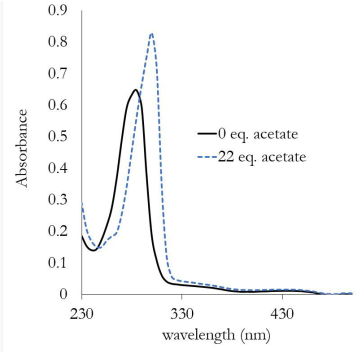
\includegraphics[width=0.8\linewidth]{figures/pub2/si_fig5.png}
    \caption{UV-Vis spectrum of 1 (10.8 $\mu$M in CD$_{3}$CN) in the absence and presence of excess acetate anion.}\label{fig:uvvis}
\end{figure}

\begin{figure}
    \centering
    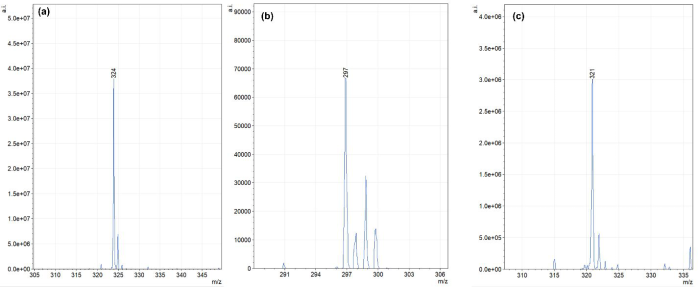
\includegraphics[width=0.8\linewidth]{figures/pub2/si_fig6.png}
    \caption{ESI-MS data for 1:1 host–guest complexes of \textbf{1} with (a) NO$_{3}^{-}$, (b) Cl$^{-}$, and (c) CH$_{3}$COO$^{-}$.}\label{fig:esi1}
\end{figure}

\begin{figure}
    \centering
    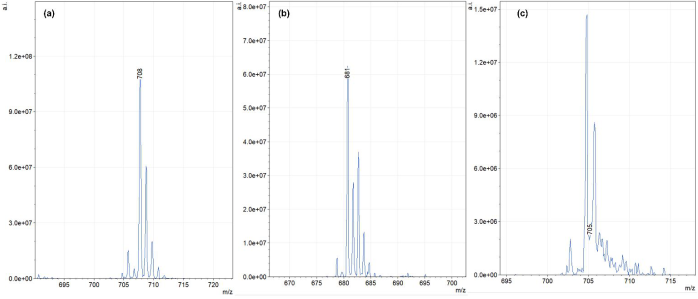
\includegraphics[width=0.8\linewidth]{figures/pub2/si_fig7.png}
    \caption{ESI-MS data for 1:1 host–guest complexes of \textbf{2} with (a) NO$_{3}^{-}$, (b) Cl$^{-}$, and (c) CH$_{3}$COO$^{-}$.}\label{fig:esi2}
\end{figure}

\begin{figure}
    \centering
    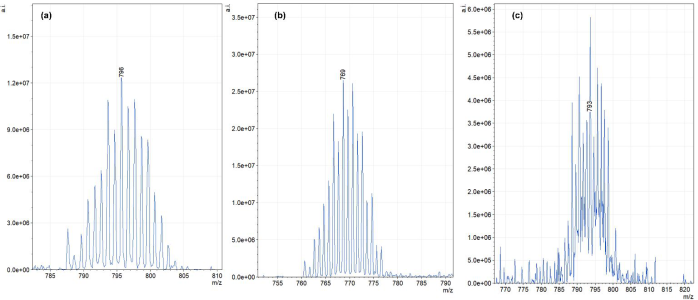
\includegraphics[width=0.8\linewidth]{figures/pub2/si_fig8.png}
    \caption{ESI-MS data for 1:1 host–guest complexes of \textbf{3} with (a) NO$_{3}^{-}$, (b) Cl$^{-}$, and (c) CH$_{3}$COO$^{-}$.}\label{fig:esi3}
\end{figure}

\begin{figure}
    \centering
    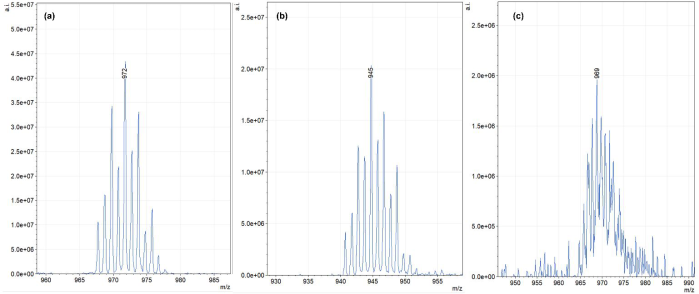
\includegraphics[width=0.8\linewidth]{figures/pub2/si_fig9.png}
    \caption{ESI-MS data for 1:1 host–guest complexes of \textbf{4} with (a) NO$_{3}^{-}$, (b) Cl$^{-}$, and (c) CH$_{3}$COO$^{-}$.}\label{fig:esi4}
\end{figure}

\begin{figure}
    \centering
    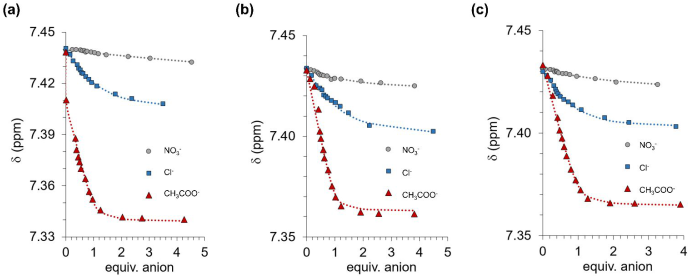
\includegraphics[width=0.8\linewidth]{figures/pub2/si_fig10.png}
    \caption{$^{1}$H NMR chemical shifting observed during titration of (a) \textbf{2}, (b) \textbf{3}, and (c) \textbf{4} ($\sim$0.1 mM in CD$_{3}$CN) with nitrate, chloride, and acetate anions. The dotted lines represent the results of non-linear fitting to a 1:1 host–guest binding model.}\label{fig:hnmr-shift}
\end{figure}